\section*{Considerações finais}
\addcontentsline{toc}{section}{Considerações finais}

Durante o desenvolvimento desse trabalho, podemos concluir que a possibilidade de soluções usando IoT é extremamente vasta e extensa. A indústria, como um todo, está aquecida e pretende absorver toda gama de demanda de eventuais serviços que envolvam esse tipo de tecnologia.

Por se tratar de um ramo da Computação que é relativamente novo (o termo foi cunhado em 1999 \cite{Kevin}, somando assim apenas 18 anos de idade no momento que este trabalho foi publicado), algumas definições não possuem uma consistência desejável e costumam divergir muito de autor para autor. O que caracteriza um certo aspecto positivo, tal que ainda há muito espaço para que mais trabalhos possam ser feitos e consolidados na indústria de IoT.

Existem tecnologias Web modernas, principalmente as baseadas em Javascript, que propiciam a construção de softwares voltado para IoT de forma fácil, produtiva, testável e manutenível.

Na elaboração desse projeto, no que tange a perspectiva da escrita do software, o maior desafio foi dos pontos de vista da elaboração arquitetural e de modelagem de dados, de forma que após as definições, a escrita do código foi relativamente simples.

\subsection{Resultados}
\label{resultados}

Como resultados deste trabalho, podemos destacar o fomento à discussão de soluções que tornem o desenvolvimento para IoT mais simples, removendo a necessidade de codificação de softwares para receber os eventos para cada projeto, conseguindo resultados em um menor tempo. E como principal ponto o desenvolvimento do software que atenda requisitos de um gateway, performático e portável, abaixo demonstraremos algumas imagens do sistema funcionando.

Na Figura~\ref{fig:raspberryDistroRaspbian} pode-se observar a aplicação sendo inicializada em um Raspberry Pi 3 Model B v1.2 (ver Figura~\ref{fig:raspberryPi3ModelB}), onde a porta TCP 3000 escutará as requisições Web e a porta TCP 1885 onde os dispositivos se conectarão pelo protocolo MQTT.
\begin{figure}[h!]
	\begin{center}
		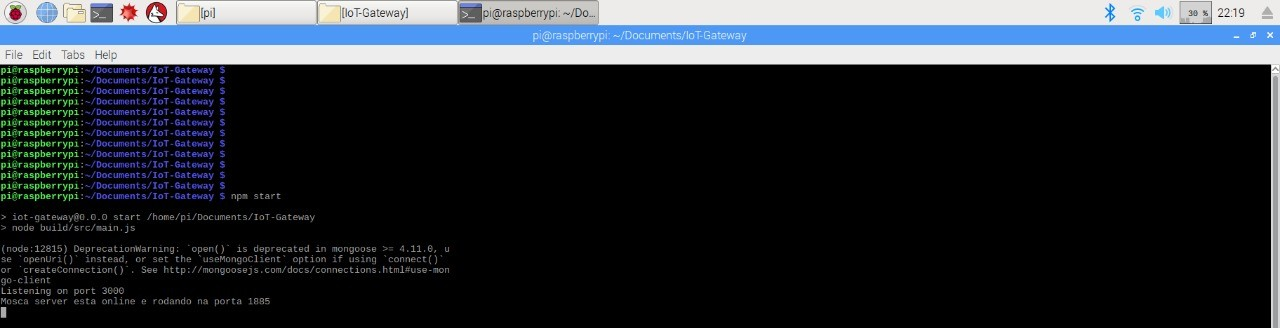
\includegraphics[width=1.085\textwidth]{./img/raspberryDistroRaspbian}
		\caption{Representação execução aplicação.}
		\label{fig:raspberryDistroRaspbian}
	\end{center}
\end{figure}

\begin{figure}[h!]
	\begin{center}
		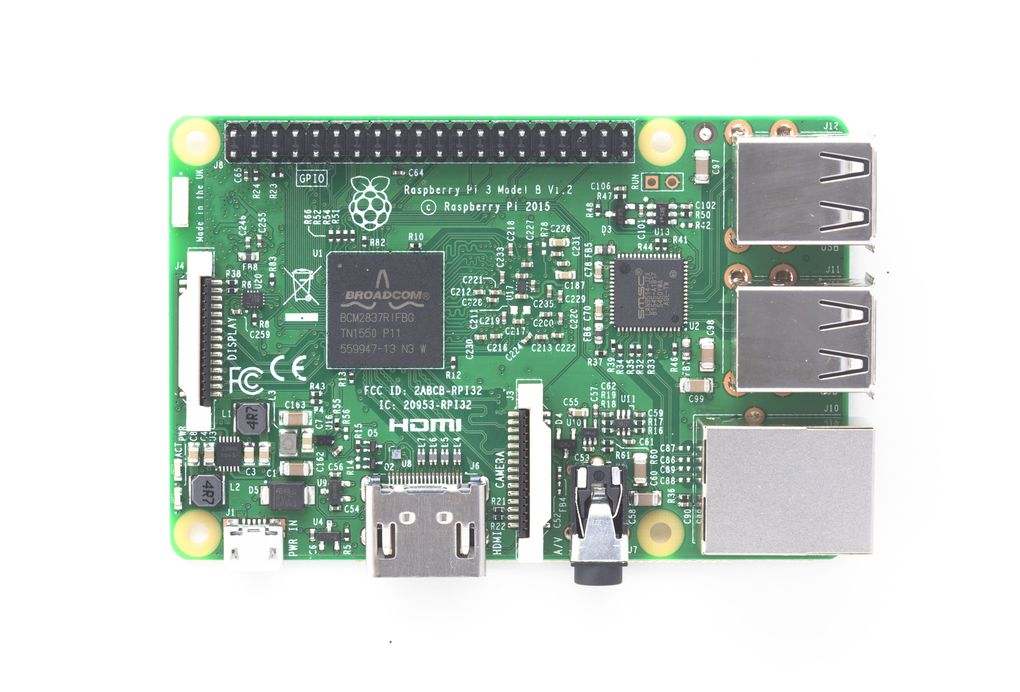
\includegraphics[width=1.085\textwidth]{./img/raspberry-pi-3}
		\caption{Exemplar do \textit{Raspberry Pi 3 Model B v1.2}, o SoC utilizado nesse trabalho}
		\label{fig:raspberryPi3ModelB}
	\end{center}
\end{figure}

Na Figura~\ref{fig:dadosBasicos} temos a tela inicial da aplicação com algumas informações a respeito da aplicação.
\begin{figure}[h!]
	\begin{center}
		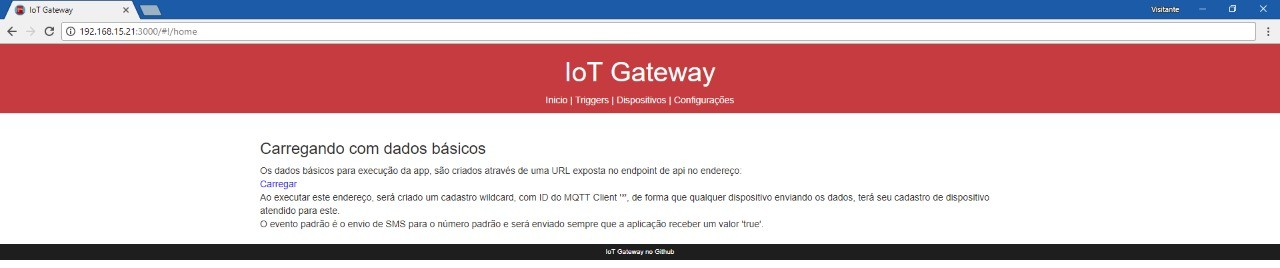
\includegraphics[width=1.085\textwidth]{./img/dadosBasicos}
		\caption{Representação visual da tela dos dados básicos.}
		\label{fig:dadosBasicos}
	\end{center}
\end{figure}

Na Figura~\ref{fig:triggerCadastrada} vemos o cadastro de uma \textit{trigger} com operação lógica de intervalo, onde o evento será executado apenas caso o valor enviado pelo dispositivo esteja entre 1 e 10. Um cenário claro de uso desta funcionalidade seria o uso do gateway para enviar notificações caso um sensor leia informações de um cenário crítico.
\begin{figure}[h!]
	\begin{center}
		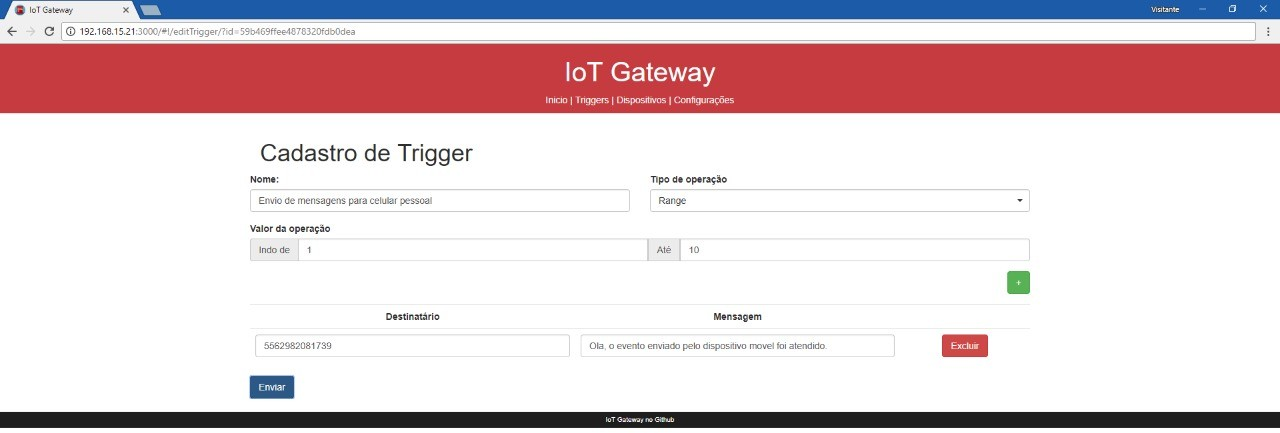
\includegraphics[width=1.085\textwidth]{./img/triggerCadastrada}
		\caption{Representação visual da tela de cadastro de trigger.}
		\label{fig:triggerCadastrada}
	\end{center}
\end{figure}

Na Figura~\ref{fig:dispositivoCadastrado} temos a listagem de dispositivos cadastrados, onde o dispositivo de nome \verb|"Celular com MyMqtt"| está cadastrado, mas sua identificar é \verb|"*"| que permite que qualquer dispositivo seja identificado por este cadastrado.
\begin{figure}[h!]
	\begin{center}
		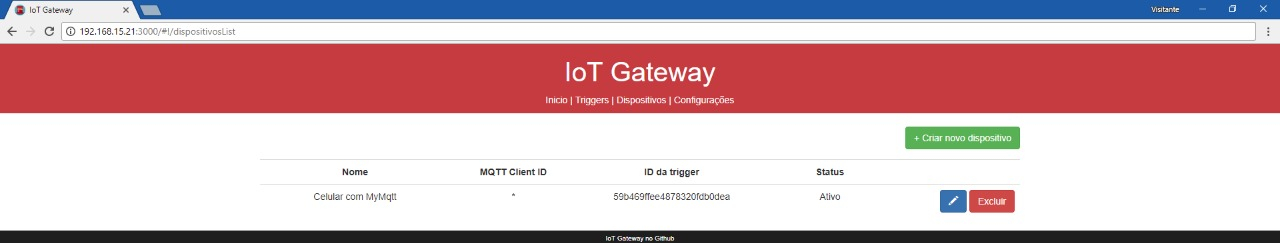
\includegraphics[width=1.085\textwidth]{./img/dispositivoCadastrado}
		\caption{Representação visual da tela de cadastro de dispositivos.}
		\label{fig:dispositivoCadastrado}
	\end{center}
\end{figure}

Na Figura~\ref{fig:aplicativoAndroidMQTT} temos um dispositivo android conectado ao gateway utilizando MQTT e enviando eventos para análise.
\begin{figure}[h!]
	\begin{center}
		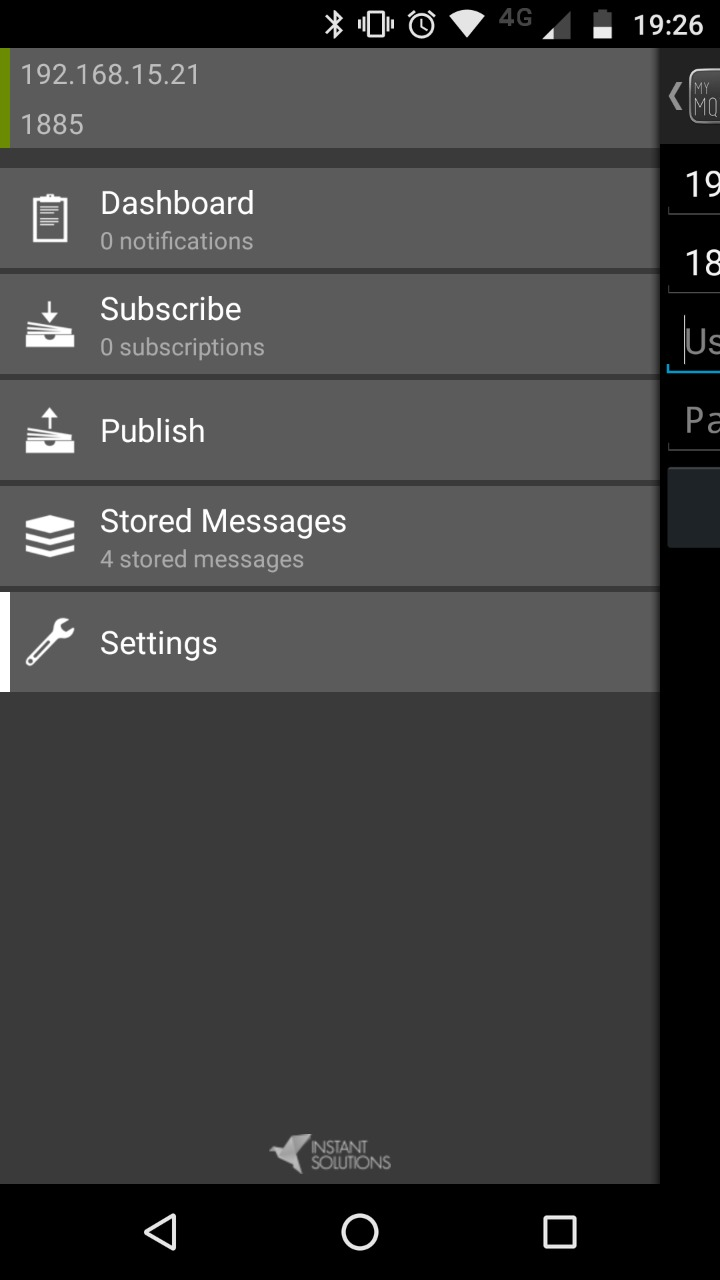
\includegraphics[width=0.85\textwidth]{./img/aplicativoAndroidMQTT}
		\caption{Representação visual do dispositivo Android utilizando protocolo MQTT.}
		\label{fig:aplicativoAndroidMQTT}
	\end{center}
\end{figure}

Na Figura~\ref{fig:eventoConsole} visualizamos o log da aplicação de 2 eventos, um em que o cenário não foi atendido, e outro em seguida onde o mesmo foi atendido e enviou o SMS.
\begin{figure}[h!]
	\begin{center}
		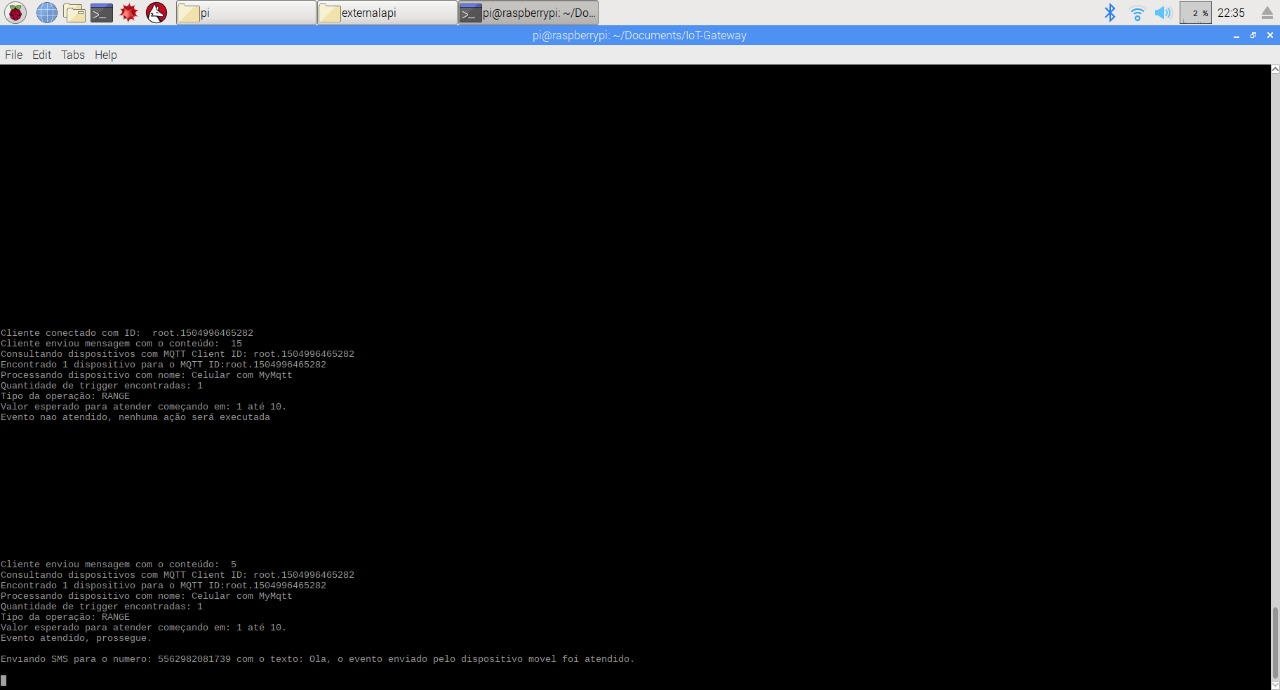
\includegraphics[width=1.085\textwidth]{./img/eventoAtendidoNaoAtendidoConsole}
		\caption{Representação visual do console ao receber eventos.}
		\label{fig:eventoConsole}
	\end{center}
\end{figure}

Na Figura~\ref{fig:smsRecebido2} o SMS recebido pelo celular após o evento atendido.
\begin{figure}[h!]
	\begin{center}
		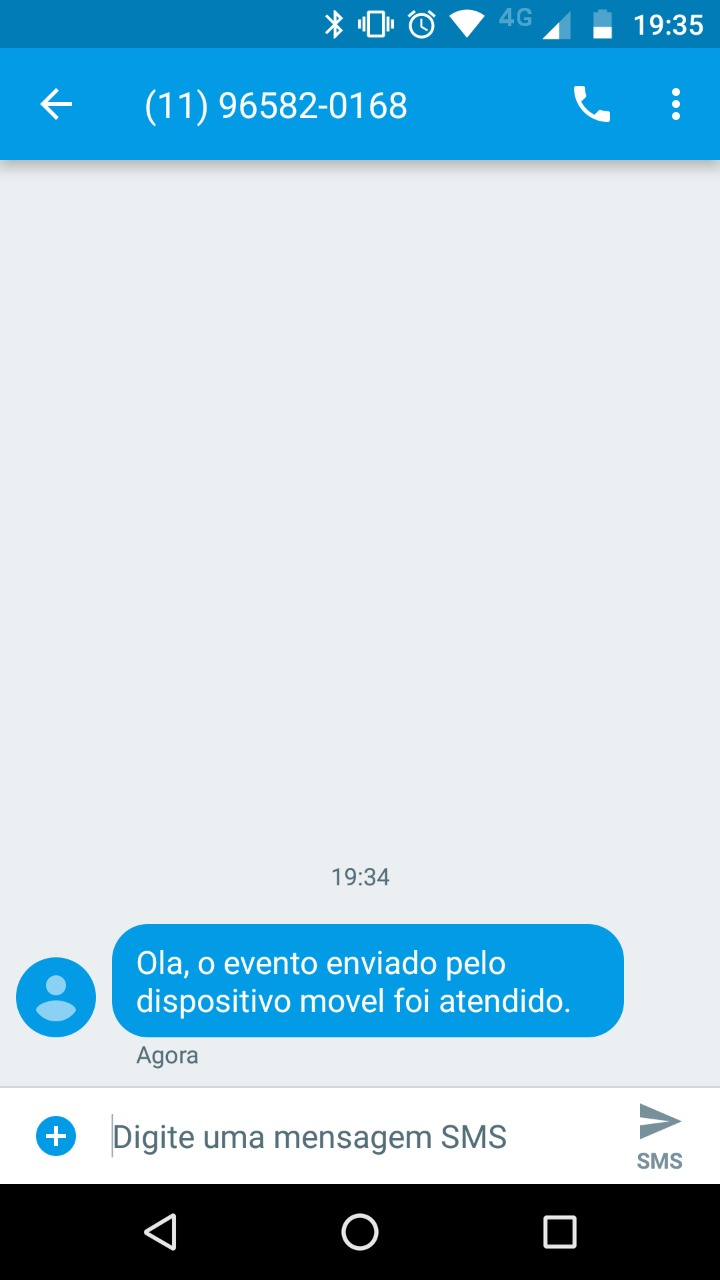
\includegraphics[width=0.8\textwidth]{./img/smsRecebido2}
		\caption{Representação visual do SMS recebido.}
		\label{fig:smsRecebido2}
	\end{center}
\end{figure}

Todos os eventos atendidos e dados recebidos são armazenados no banco de dados da aplicação para consulta posterior.

\subsection{Trabalhos futuros}
\label{trabalhosFuturos}

Como trabalhos futuros, destacamos um suporte a mais protocolos de comunicação com dispositivos e outras funções existentes em outros gateways, como a transmissão posterior das informações armazenadas para a cloud e suporte a novos eventos como, envio de email, ligações e até envio de informações para outros dispositivos, assim tornando o gateway como um dispositivo não só passivo, mas como atuante na rede em que eles está inserido.





